\externaldocument{capitulo05}

\chapter{\hspace*{3pt} Avaliação}
\label{chap:avaliacao}

%\section{\hspace*{3pt} Introdução}\label{sec:introducao}

A noção de qualidade em modelos conceituais, o seu significado e como alcançá-la, ainda geram inúmeros debates por parte dos especialistas \citep{teeuw:1997.quality}. 

As primeiras pesquisas simplesmente listam propriedades desejáveis que podem ser encontrados em ``boas" representações conceituais \citep{navathe:1992.conceptual}.Definições, quando administradas, são vagas e complicadas, e não existe qualquer estrutura subjacente que ajude a compreender as propriedades e como se relacionam umas com as outras. O resultado é um conjunto de avaliações \textit{ad hoc} de representações, e pouco consenso sobre o que faz uma representação ser ``boa" \citep{moody:1998.improving}. 

Segundo \citet{nelson:2012.conceptual}, diferentes \textit{frameworks} tentam solucionar a problemática acerca da qualidade das representações de modelagens conceituais e das qualidades dos processos de modelagens conceituais. Duas estruturas se destacam entretanto: A primeira é um \textit{framework} introduzido por Lindland, Sindre, e Sølvberg (LSS) \citep{lindland:1994.understanding} baseado na teoria semiótica de Morris, e o segundo é um \textit{framework} desenvolvido por Wand e Weber com base em teoria ontológica da Bunge (o modelo representacional Bunge-Wand-Weber: BWW) \citep{wand:1990.ontological}. 

O \textit{framework} sugerido por \citet{wand:1990.ontological} é um processo atuante durante a modelagem, o que poderia interferir em nossas análises, por esse motivo optamos por utilizar a proposta de \citet{lindland:1994.understanding}, focada na análise do resultado do processo de modelagem. Em sua proposta três tipos de qualidade são introduzidos:
 
\begin{itemize}
\item \textbf{Qualidade Sintática}: é o quanto um modelo conceitual e sua representação se correspondem.  O conjunto de erros sintáticos contém todas as declarações que podem ser expressas no modelo, mas (pode) não (ser feita) na língua.\\
\item \textbf{Qualidade Semântica}: é o grau de correspondência entre o modelo conceitual e o mundo real. Se um modelo contém declarações que não têm correspondência no mundo real, o modelo é inválido, no caso contrário, o modelo é incompleto.\\
\item \textbf{Qualidade pragmática}: é o grau de correspondência entre o modelo conceitual e sua interpretação (individual), ou seja, até em que grau um modelo é compreendido.
\end{itemize}

A qualidade sintática não será relevante neste trabalho, pois assumimos que os conceitos podem ser capturadas em uma linguagem adequada. E, a exemplo do que foi proposto em \citep{teeuw:1997.quality} para capturar a qualidade semântica e qualidade pragmática, utilizaremos os seguintes critérios de qualidade:

\begin{enumerate}
\item Abrangência: Os conceitos devem ser expressivos o suficiente para capturar todos os "aspectos essenciais" do mundo real.
%\item Inerência (propriedade): Os conceitos deve ser diretos e se concentrar em aspectos essenciais.
\item Clareza: Os conceitos e regras, bem como sua aplicabilidade, devem ser compreensíveis, sem dispêndio de muito tempo e esforço.
\item Consistência: Os conceitos não deve entrar em conflito uns com os outros nas representações dos aspectos do mundo real. Consistência implica não-ambiguidade: um conceito tem apenas um único sentido no mundo real.
\item Modularidade: aspectos independentes do mundo real devem ser capturados por diferentes conceitos, e aspectos fortemente relacionados deve ser representados por conceitos relacionados.
%\item Generalidade: Os conceitos deve ser tão independente quanto possível, a partir de qualquer aplicativo específico ou domínio de aplicação.
\end{enumerate}

Os critérios apresentados abrangem a qualidade ``externa" dos conceitos, àquelas utilizadas para a satisfação dos usuários, e a qualidade ``interna", as propriedade intrínsecas dos conceitos. 

\section{\hspace*{3pt} Metodologia}
\label{sec:avaliacaoMetodologia}

Procuramos avaliar é se a utilização do processo proposto neste trabalho, e suas teorias subjacentes, promovem uma melhoria nos modelagem conceitual e, por conseguinte, em sua representação correspondente. 

\citet{castro:2010.abordagem} aponta as dificuldades existentes para a mensuração de propriedades qualitativas em modelos conceituais, e explica que, tal análise demanda a aplicação das teorias e técnicas propostas em uma situação real, ou em um estudo de caso. 

\subsection{\hspace*{3pt}O Estudo de Caso}

Para o estudo de caso apresentado, optamos por uma abordagem pictográfica para a apresentação do contexto. \citet{souza:1998.discurso}, argumenta que a referencialidade sustenta a possibilidade de leitura da imagem e, por outro lado, reafirmam o seu \textit{status} de linguagem. 

A descrição textual, conforme \citet{heuser:2001.projeto} e \citet{machado:2009.projeto}, fornece importantes dicas acerca de quais objetos, relações e atributos são relevantes para o contexto. Trabalhos como o de \citet{castro:2010.abordagem} e \citet{leao:2012.construcao}, apresentam abordagens para a modelagem conceitual pautada em descrições textuais. Neste sentido as imagens tentaram favorecer a explanação do contexto e de suas atividades, deixando os participantes livres para a interpretação do contexto sem, no entanto, transmitir quaisquer informações explicitas.

Para participar desta fase da pesquisa, foram convidados analistas de sistemas, com conhecimentos na área de desenvolvimento de software, especificação de software ou Banco de Dados.

Com o objetivo de avaliar a aplicação do processo OR, dividimos os participantes em dois grupos, o grupo A e o Grupo B, e em cada grupo realizamos duas rodadas de modelagens, com o intuito de responder a questões distintas.

No grupo A, estávamos interessados em avaliar se o processo OR influenciaria a descoberta de conceitos pertinentes a um determinado contexto, e se essa representação seria mais completa.

No grupo B, nosso intuito era analisar se, uma vez apresentados ao processo, os modeladores utilizaram as fases descritas para elaboração novos modelos, mesmo quando não solicitado que o utilizassem.

Na primeira rodada, para cada participante, em ambos os grupos, uma série de imagens foram apresentadas, cada imagem continha uma cena peculiar, que apresentava o contexto de uma livraria e em algumas delas, havia a sugestão da realização da compra de livros.

Após essa exposição, cada participante foi instruído a elaborar um modelo conceitual, utilizando o linguagem de sua preferência para a representação deste contexto. O modelo deveria expor o contexto, com toda riqueza de detalhes (conceitos, características e relações) que o participante julgasse necessário para expressá-lo, em especial sua atividade fim, sem ambiguidades. 

O grupo A, deveria executar essa modelagem sem o auxílio do processo OR, ao passo que o grupo B foi apresentado ao processo proposto neste trabalho, e deveria efetuar sua elaboração considerando as fases de aquisição, categorização e representação dos conceitos percebidos.

Na segunda rodada, o grupo A foi apresentado ao processo, e lhes foi solicitado que considerando o exposto, revisassem o modelo criado previamente, refazendo-o caso julgassem necessário.

Enquanto que ao grupo B, um novo contexto com uma tarefa específica, desta vez com imagens mais explícitas, foi apresentado e solicitado um modelo que fosse capaz de representá-lo.

Para efetuar a captura de dados processo de modelagem foi gravado, e as gravações analisadas.

\subsection{\hspace*{3pt} Avaliação dos Processos e Modelos}

Esta avaliação se propõe a entender como os participantes entendem o contexto e que conceitos são capazes de alcançar através da observação das imagens e reflexão sobre o contexto e suas atividades. 

\subsubsection{\hspace*{3pt} Grupo A}

O primeiro participante do grupo A, que chamaremos de A1, é analista de sistemas e possui 10 anos de experiência, tendo trabalhado para empresas do setor público e privado. Porém, apenas atualmente desenvolvendo para uma instituição federal, tem atuando na área de análise e modelagem de requisitos.

Em sua modelagem, o analista A1, observou que o contexto tratava-se de uma livraria e seu primeiro conceito destacado no modelo foi o de livro. Porém no decorrer na elaboração, deu-se conta de que o conceito livro, era um termo com intensão muito específica, e que embora trouxesse clareza para seu modelo, sua abrangência era muito limitada, o que o fez optar por outro conceito, o de publicação, e associou ao conceito de tipo de publicação. O tipo de publicação, afim de trazer consistência e modularidade, demandaria a especificação dos tipos de publicação, no entanto o analista A1 não o fez, deixando-o subjetivo. 

O analista A1 também entendeu que toda publicação estava localizada em uma seção e também deveria ter um autor, e ocasionalmente seria comprada por um cliente. O conceito cliente se evidenciou com mais facilidade, porém ao retornar as imagens que descreviam o contexto, o analista sentiu necessidade de representar o conceito compra e escolheu o símbolo \textit{adquire} para  nomeá-lo em um primeiro momento, alterando-o para \textit{compra} pouco tempo depois. Aqui novamente pode-se perceber a escolha por um conceito que transmitisse maior clareza e abrangência. Clareza porque \textit{adquirir} não deixa claro como se deu a aquisição e abrangência porque \textit{compra}, evidencia o especto essencial da atividade fim de uma livraria.

Finalizou seu modelo, detectando a necessidade de acrescentar o conceito tipo de pagamento em relação a compra, afim de melhorar a modularidade do conceito de compra. 

Nenhum outro conceito foi apresentado ou quaisquer características listadas, embora se possa perceber através das suas escolhas acerca de quais símbolos utilizar para representar os conceitos que características distintas foram levadas em consideração, por exemplo para a troca do conceito livro por publicação ou o conceito aquisição por compra.

A Figura \ref{fig:modeloA1001} demonstra o resultado final do modelo do analista A1, após a primeira rodada.

\begin{figure}[!ht]
    \centering
    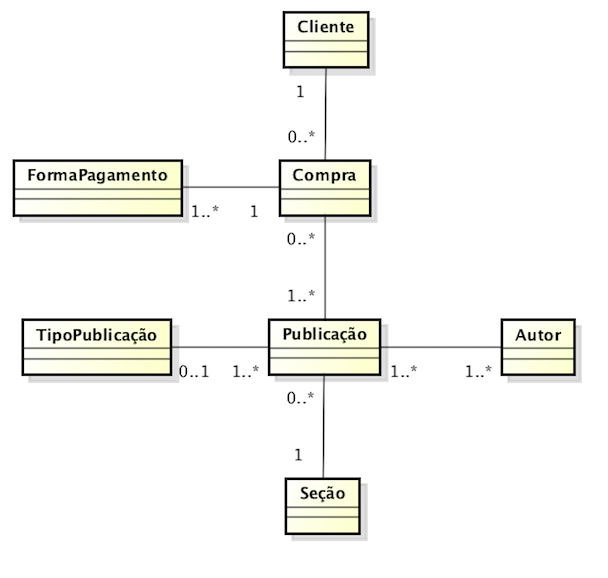
\includegraphics[width=\textwidth]{imagens/Modelo_001_Aline_Macena.png}
    \caption{Modelo gerado pelo analista A1 sem o Processo OR}
    \label{fig:modeloA1001}
\end{figure}

Após a apresentação do processo OR, o analista A1 foi convidado a rever sua modelagem, no entanto, sentiu necessidade de efetuar poucas mudanças na distribuição dos conceitos, adicionando apenas o conceito editora.

Porém, sua nova análise apontou a necessidade de elencar características que definem cada conceito. Podemos perceber em seu novo modelo, Figura \ref{fig:modeloA1002}, que algumas dessas características foram adicionadas como atributos seguindo o paradigma da linguagem UML e outros como comentários.  

Outra aspecto alterado foi a descrição dos papeis executados por cada conceito, favorecendo a clareza desses conceitos. Algumas características, como as representadas pelos símbolos \textit{livro} e \textit{revista}, apesar de explicitados não se tornaram novos conceitos no modelo, algo que poderia favorecer a consistência e a modularidade do modelo final.

\begin{figure}
    \centering
    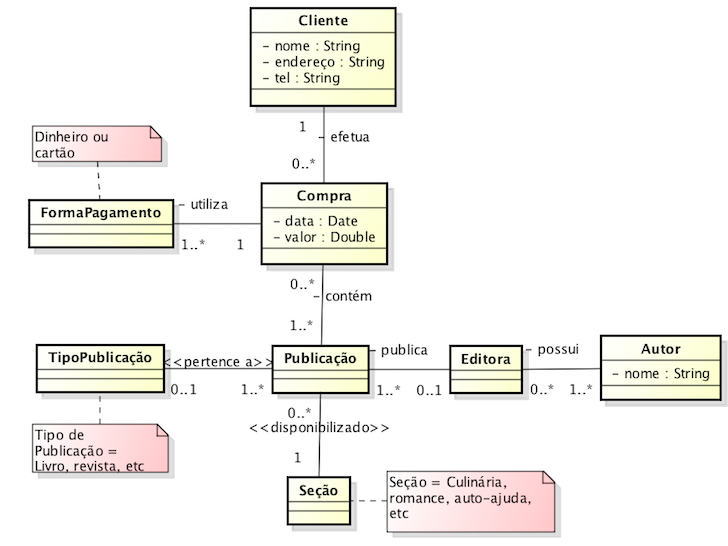
\includegraphics[width=\textwidth]{imagens/Modelo_002_Aline_Macena.png}
    \caption{Modelo gerado pelo analista A1 com o Processo OR}
    \label{fig:modeloA1002}
\end{figure}

O segundo participante do grupo A, que chamaremos de A2, possui formação e experiência acadêmica apenas, sem quaisquer experiências no mercado de trabalho. 

O analista A2 iniciou sua modelagem através do conceito item, e representou explicitamente suas características. Em seguida definiu os conceitos livro e revista como conceitos de menor abrangência em relação ao conceito item. Segundo a linguagem UML, escolhida para representar o contexto, essa configuração caracteriza uma herança. O analista continuou, apontando as características dessas heranças e relacionou o conceito pai, item, ao conceito pedido através de uma relação. 

O símbolo \textit{item} embora possua uma grande abrangência, sozinho, não traz ao modelo clareza, consistência ou modularidade, mas ao ser definido como um conceito pai, de livro ou revista, não só resolve esses problemas, como também demonstra que para o analista A2 ambos os conceitos são tipos de itens, isto é, evidencia sua categorização racional. 

O analista também identificou na sequência o conceito item estoque; pedido do cliente, cliente, pedido fornecedor. Declarando as relações de herança de pedido cliente e pedido fornecedor ao conceito pedido; e uma relação direta entre item estoque e item; e outra relação direta entre cliente e pedido cliente. Identificou o conceito vendedor e declarou uma herança, considerando cliente e vendedor, como filhos em relação ao conceito pessoa física. Pessoa jurídica, após ser declarada, foi adicionada como um conceito filho, junto com pessoa física ao conceito pessoa.

Podemos perceber que determinados conceitos, demandam outros conceitos. Como percebido na modelagem do analista A2, onde compra é feita por cliente, que efetua um pedido, que possui item de pedido, que é retirado do estoque.

Da mesma maneira aqui, a compra gera baixa no estoque, que precisa ser reposta por um fornecedor, através de um pedido de compra onde constam itens para a reposição.

Pessoa jurídica deu origem a um conceito filho, denominado fornecedor. E este colocado em relação direta com conceito pedido fornecedor. Todas as características, de cada um dos conceitos, foram listadas, o que indica o favorecimento de uma melhor descrição do contexto.

A analise do contexto efetuada pelo analista A2, revelou conceitos que não estavam implícitos nas imagens, como fornecedor, estoque, mas que foram evidenciadas ao considerar os conceitos presentes no contexto. Seu modelo, está representado pela Figura \ref{fig:modeloA2001}.

\begin{figure}[!ht]
    \centering
    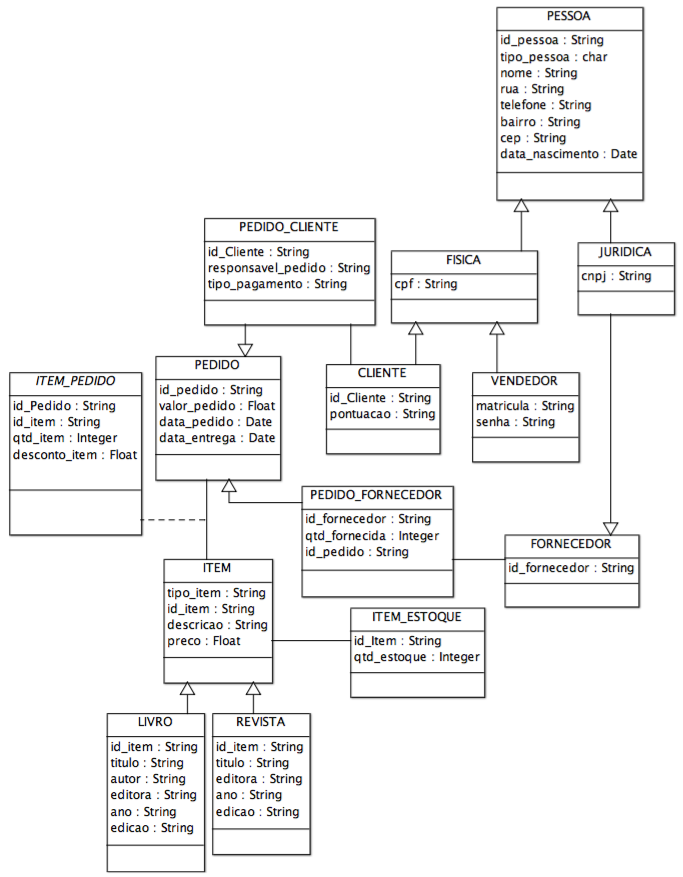
\includegraphics[width=\textwidth]{imagens/Modelo_001_Vanessa_Sales.png}
    \caption{Modelo gerado pelo analista A2 sem o Processo OR}
    \label{fig:modeloA2001}
\end{figure}

Após ser apresentado ao Processo OR, o analista foi convidado a rever sua modelagem. O analista apresentou certa confusão ao repensar o domínio, e não parecia estar muito certo sobre como proceder na passagem pelo processo. Confusão que foi sanada após alguns questionamentos acerca das etapas, e apresentação de alguns exemplos. No final deste, o analista optou por refazer o modelo utilizando metamodelo Entidade-Relacionamento.

Com está abordagem, o analista utilizou-se da marcação de relacionamento típico do metamodelo E-R, o losango, para representar relações que julgava necessárias. 

Nesta nova abordagem, o analista começou sua apresentação através do conceito livro, para qual foram definidas as mesmas características listadas no modelo anterior. Porém percebemos que a utilização do processo OR, o levou a analisar quais outras características são essenciais para o conceito livro, dentro do contexto livraria,  fazendo com que fosse representado a relação de pertencimento a uma coleção. Além de outras características definidoras do mesmo, em uma relação de posse, a citar: numero de páginas, tipo de página, capítulos, imagens, orelha, capa, contracapa, categoria. Todas após definir a relação de posse.

Embora essas características não tenha sido representadas dentro do conceito livro, como atributos fica evidente que as características adicionam clareza e modularidade ao conceito.

Para o conceito revista, segundo a ser representado, a exemplo do livro, o analista atribuiu as mesmas características do primeiro modelo. Em seguida adicionou outras características em uma relação de posse, exceto por substituiu capítulos por colunas, e ter adicionado seções, anúncios e índice, foram as mesmas atribuídas em livro. 

A Adição da última característica, índice, no conceito revista o fez retornar ao conceito livro e também adicionar índice e subtítulo como características.

Após suas representações, o analista generalizou os conceitos, adicionando ambos como filhos do conceito item, e nomeando os papeis . Transformando a abordagem anterior \textit{top-down},  em uma abordagem \textit{bottom-up}, isto é, definindo primeiro os conceitos de menor abrangência e a partir deles, os conceitos de maior abrangência.

A partir deste ponto, o analista apenas replicou o modelo anterior, porém acrescentando as relações entre os conceitos e nomeando os papeis, como podemos verificar na Figura \ref{fig:modeloA2002}.

\begin{figure}[!ht]
    \centering
    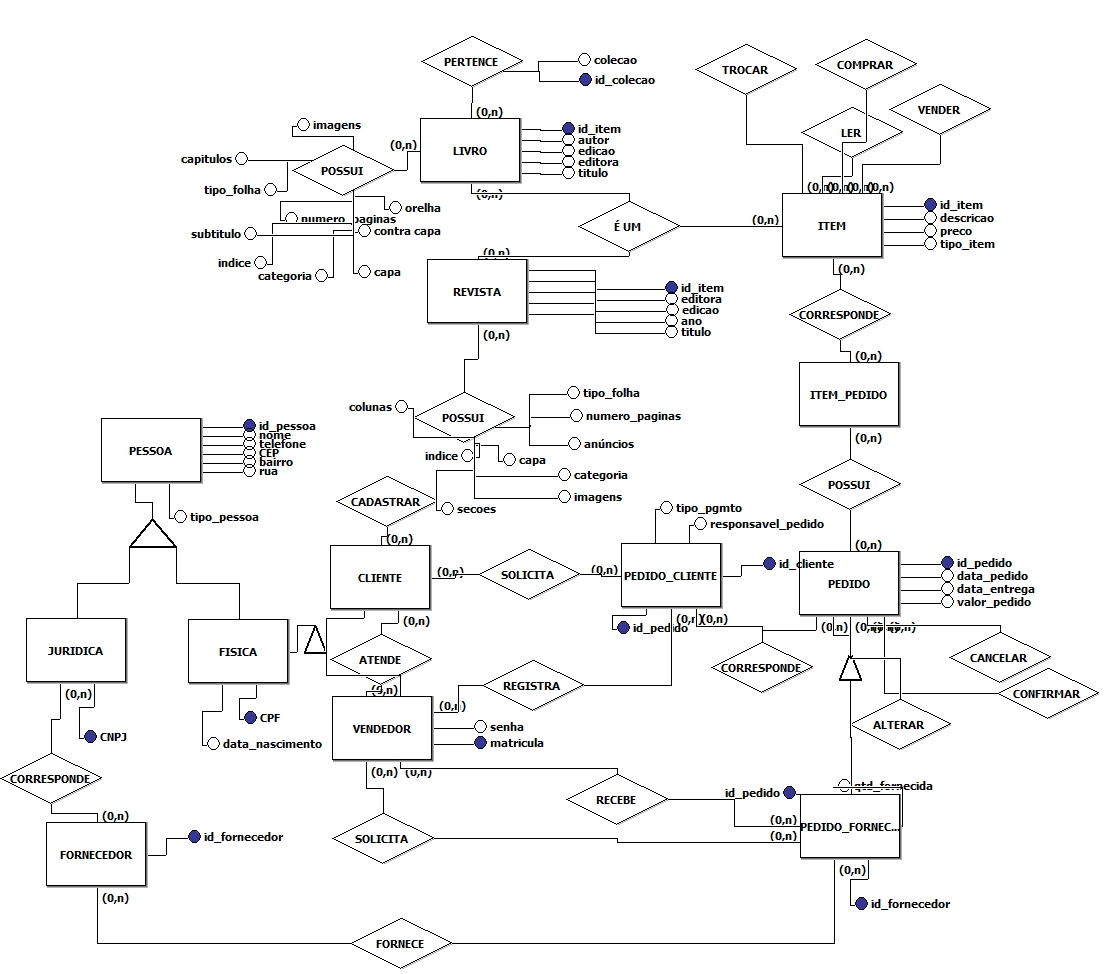
\includegraphics[width=\textwidth]{imagens/Modelo_002_Vanessa_Sales.jpg}
    \caption{Modelo gerado pelo analista A2 com o Processo OR}
    \label{fig:modeloA2002}
\end{figure}

\subsubsection{\hspace*{3pt} Grupo B}

No grupo B, o primeiro analista, aqui chamado de analista B1, declarou possuir 10 anos de experiência na área de TI e que mais da metade de suas atividades, possuem relação ou estão diretamente ligadas à modelagem conceitual.

Após ser apresentado ao processo OR, o analista B1 iniciou sua tarefa de modelagem e identificou sem maiores problemas o contexto que deveria representar. 

Sua representação iniciou-se pelo conceito livro, e foi seguido pelos conceitos que representavam a atividade fim do contexto, isto é, a venda de livros. Em sua representação, o analista B1 adicionou as características que julgou mais importantes à todos os conceitos, e através dos construtos da UML, representou as relações de composição e agregação existentes entre os conceitos identificados, isto é, as relações parte-todo.

Somente após essa representação mais imediata da atividade fim do contexto, o analista expandiu sua representação, porém trazendo mais elementos que compunham a atividade de venda. Nesta expansão, uma herança foi adicionada, na forma do conceito mais geral, representado pelo símbolo \textit{pessoa} e três conceitos mais individuais, representados pelo símbolos \textit{vendedor}, \textit{autor} e \textit{cliente}.

Apesar de utilizar o Processo OR, o analista não distinguiu de maneira clara os tipos de publicações existentes nas imagens e nem considerou a reposição do estoque, embora tenha declarado a existência da característica que remeteria e este conceito. Escolha que, considerando os critérios de qualidades utilizados, não favorece o modelo quanto a modularidade e abrangência. A definição de um conceito categoria, com a característica de nome, não favorece a qualidade de clareza.  

Uma conclusão possível seria que o analista optou por uma abordagem direta, focada na atividade fim do contexto, representando apenas os conceito imediatos, dentre os quais, apesar de haver revistas nas prateleiras, não havia imagem que mostrasse a compra de uma revista.

Fato que pode reforçar essa analise, é a representação dos conceitos autor, editora e categoria, relacionados com o conceito livro. Conceito que estava imediatamente representada nas imagens de prateleiras e de compras.

Outro ponto a se destacar, é o fato de que para os conceitos representados, o analista atribuiu características que segundo sua analise eram essências para a definição destes mesmos conceitos

\begin{figure}[!ht]
    \centering
    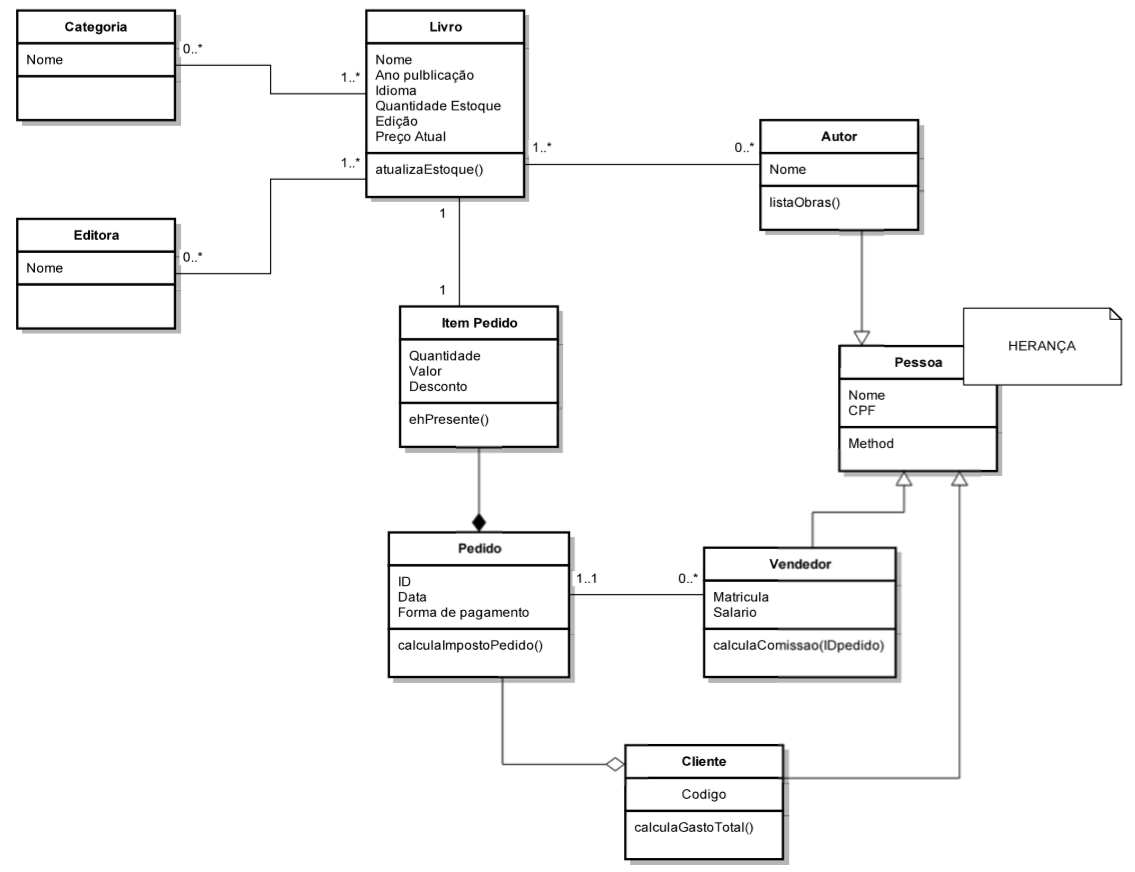
\includegraphics[width=\textwidth]{imagens/Modelo_001_Igor.png}
    \caption{Modelo gerado pelo analista B1 com o Processo OR}
    \label{fig:modeloB1001}
\end{figure}

Assim que o analista declarou o fim de seu modelo, foi lhe solicitado que, realizasse uma nova tarefa de modelagem. Porém sem a utilização processo apresentado neste trabalho.

O novo contexto representava a aquisição de ingressa para um espetáculo teatral. Contexto que foi interpretado de imediato pelo analista B1, e seu conceito primário, foi exatamente o de um espetáculo.

Em sua representação, o analista B1 foi capaz de destacar conceitos como personagem, artista, produtor executivo e patrocínio, conceitos que não eram sugeridos através das imagens e que, apesar de se relacionarem com o contexto, não remetiam à tarefa de comprar de ingresso.

A Representação dos conceitos pode indicar a permanência, de maneira subjetiva, das faixas que compunham o processo OR, em especial a fase 02, que diz respeito a racionalização. Suspeita esta, sustentada pela existência de conceitos que na verdade poderiam ser alcançados definindo as características essenciais de um espetáculo.

Quando sua representação é analisada sob os critérios de qualidade designados, apenas se considerarmos os tipos de espetáculos que podem estar em cartaz em um teatro, o critério de modularidade não é atendido. No entanto, a representação possui clareza, abrangência e consistência.

\begin{figure}[!ht]
    \centering
    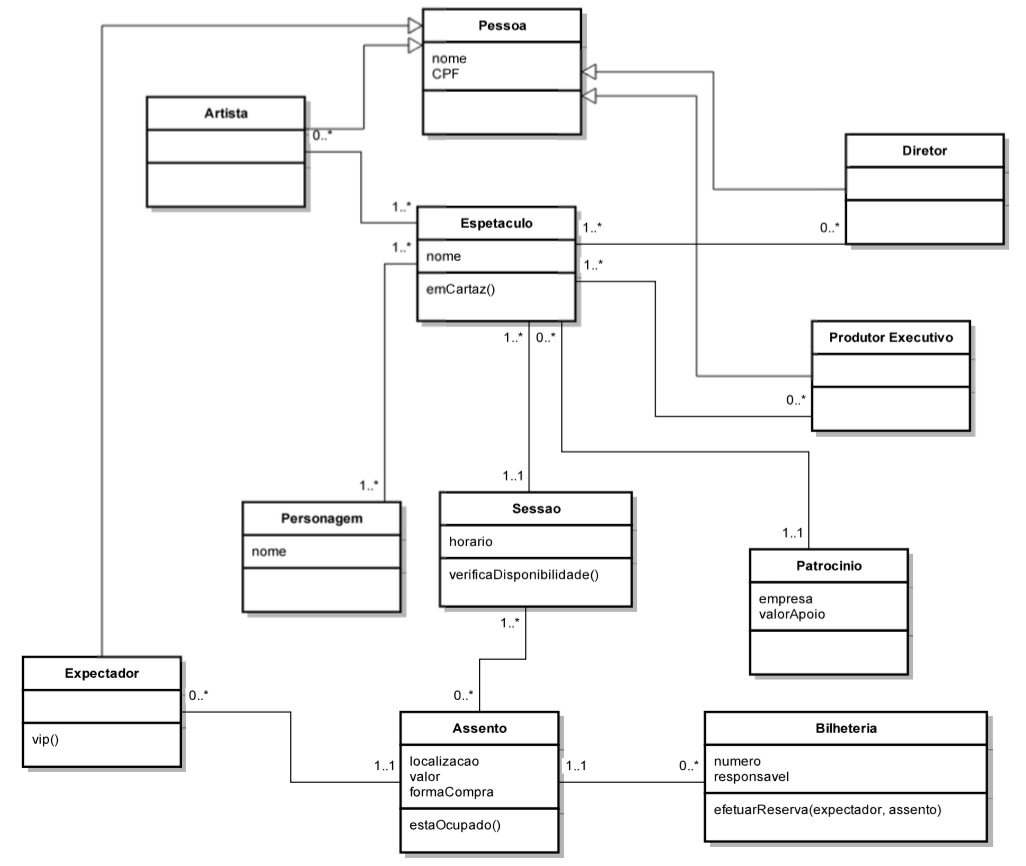
\includegraphics[width=\textwidth]{imagens/Modelo_002_Igor.png}
    \caption{Modelo gerado pelo analista B1 sem o Processo OR}
    \label{fig:modeloB1002}
\end{figure}

O analista B2, possui experiência de dez anos na área de desenvolvimento de \textit{softwares} e tem experiência com bancos de dados. Optou para sua representação, a descrição textual e em sua elaboração do modelo, começou sua representação através do conceito livro. Destaca-se o fato de que, ao descrever as características do conceito livro, declarou o tempo de entrega.

Sua abordagem seguiu a conexão de conceitos esperada, isto é, uma compra, tem itens e esses itens precisam ser pagos. Seu modelo reflete esse pensamento ao definir os conceitos pedido, item do pedido e pagamento. 

Para cada conceito, o analista B2 listou cada uma de suas características, declarando as aquelas que efetivamente uniam um conceito à outro. Durante sua modelagem, pôde-se observar alguns minutos onde parecia analisar o próximo conceito a ser inserido e se as características listadas, representavam bem o conceito já representado.

Este analista também, embora defina uma característica quantidade em estoque, não representa a possibilidade da existência de um fornecedor, assim como não considera existência de outros tipo de publicações nas imagens que definem o contexto. 

Podemos perceber que, apesar de nenhuma imagem fazer alusão a compras \textit{on-line}, o analista B2 considerou sua representação para um ambiente web. Essa analise é motivada pela existência do conceito endereço e pela característica tempo de entrega, atribuída ao conceito livro.

O que nos leva a crer que, também em busca de uma objetividade, o analista apenas considerou a atividade fim do contexto. 

Sua representação textual encontra-se logo abaixo:

\begin{quote}
Entidades (classes):\\
Livro {\\
   - isbn\\
   - titulo\\
   - descrição\\
   - quantidadeEstoque\\
   - preçoVenda\\
   - tempoEntrega\\
   - categoria (Referência para classe categoria)\\
}\\
Categoria {\\
   - id\\
   - nome\\
   - descrição\\
}\\
Cliente {\\
   - cpf\\
   - nome\\
   - endereço (Referência para classe endereço)\\
   - telefone\\
   - email\\
}\\
Endereço {\\
   - rua\\
   - cep\\
   - bairro\\
   - numero\\
   - cidade\\
   - estado\\
   - país\\
   - complemento\\
}\\
Pedido {\\
  - numero\\
  - data\\
  - endereçoEntrega (Referência para classe endereço)\\
  - status\\
  - cliente (Referência para classe cliente) \\
}\\
Pagamento {\\
  - numero\\
  - valor\\
  - data\\
  - pedido (Referência para a classe Pedido)\\
  - lista de item do pedido (Referência para classe itemPedido)\\
}\\
itemPedido {\\
   - livro (Referência para classe livro)\\
   - quantidade\\
}

\end{quote}

Após a finalização da elaboração do modelo, o novo contexto lhe foi apresentado e sua representação iniciou-se com o conceito espetáculo. O analista apontou seis conceitos explicitamente e cada uma das características que julgou necessária, incluindo as relações que teriam, no entanto, comentou que conceitos como funcionário ou categoria de espetáculos poderiam ser representados, mas não sentiu necessidade de explicita-las visto que sua representação, apresentava minimamente o conceito.  

Considerando a tarefa especifica de compra de ingresso, a representação do analista atende aos critérios de qualidade listados. 

\begin{quote}
Entidades (classes):\\
Espetáculo {\\
    - id\\
    - nome\\
    - tempo de duração\\
}\\
Cliente {\\
    - id\\
    - nome\\
    - endereço (Ref. para classe endereço)\\
}\\
Endereço {\\
    - rua\\
    - cep\\
    - bairro\\
     ....\\
}\\
Sala {\\
    - id\\
    - nome\\
}\\
Sessão {\\
    - sala (Ref. para classe sala)\\
    - espetáculo (Ref. para classe espetáculo)\\
    - data/hora início\\
    - data/hora fim\\
    - preço\\
    - número de assentos disponíveis\\
}\\
Compra {\\
    - sessão (Ref. para classe sessão)\\
    - cliente (Ref. para classe cliente)\\
    - forma de pagamento\\
    - assento comprado\\
}\\
\end{quote}

Podemos observar, para ambos os analistas do Grupo B, que a escolha do conceito de maior abrangência, em detrimento de uma maior especificação - como por exemplo o conceito apresentação, visto que a imagem destacava um grupo de balé - pode ser reflexo do entendimento de que uma peça de teatro e um concerto também representam um espetáculo. Evidenciando uma escolha por um conceito mais geral para tornar o modelo mais genérico. De encontro com essa observação, podemos ressaltar o fato de que o analista B1 entende que espetáculos são compostos por atores e personagens.

O analista B1 relatou após a elaboração do modelo conceitual, de maneira informal, que ao utilizar o processo Objeto-Representação percebeu que muitas de suas assunções, feitas de maneira automática, foram reconhecidas no processo e que o mesmo ajuda a focar nos conceitos importantes, sem se aprofundar em demasia ou em escassez, o que pode significar um ganho de tempo na busca da melhor maneira de representar um conceito.

O analista B2, reiterou após a execução da tarefa que regras não estavam explicitas em seu modelo, tais como verificar se haveria assento disponível ates de efetuar a venda.

\section{\hspace*{3pt} Conclusão}
\label{sec:conclusaoAvaliacao}

Neste capítulo foi apresentado a metodologia para avaliação da proposta deste trabalho, afim de averiguar se o Processo Objeto-Representação era capaz de guiar os modeladores através dos conceitos e de suas concepções. Nosso objetivo principal foi comparar os resultados dos modelos criados pelos analistas sem a aplicação do método, com os modelos resultantes com sua aplicação, afim de perceber a definição de conceitos e características que antes não haviam sido representados em uma análise qualitativa. 

Observamos que a descoberta de novos conceitos foi possível, mas apesar disto, nem todos passaram a figurar exatamente como conceitos nos modelos. Alguns foram listados como características de conceitos já existentes. 

Da mesma forma, buscou-se observar se após o contato com o processo, haveria a continuidade da reflexão acerca da formação dos conceitos, em busca da melhor representação do mesmo. A conclusão desta avaliação, embora não possa ser percebida de maneira explicita nos modelos resultantes, pode ser observada, na escolha proposital de conceitos mais gerais para representar o contexto, diante de uma tarefa específica.

Finalmente, a avaliação aqui proposta, sugere que a adoção de um processo que explicita o reconhecimento do objeto e os caminhos percorridos por nosso intelecto até sua representação, podem ajudar modeladores a pensarem os contextos que estão tentando representar, levando-os a considerarem conceitos e características até então não foram considerados. A avaliação sugere também, que o Processo ao analisar um dado conceito inserido no seu contexto, pode auxiliar o modelador na escolha do símbolo para representar este conceito, no modelo conceitual que está sendo elaborado.